\chapter{定态Schr\"{o}dinger方程}
    \section{定态和分离变量法}
    列出Sch\"{o}dinger方程后的下一步就是解出系统对应的波函数, 首先我们应该从最最初等的分离变量法来解方程, 毫无疑问我们只能通过它来\uwave{猜出}解空间
    的一小部分子集, 但是这种方法得出来的解却具有非常重要的物理意义, 后面的一系列讨论都默认势能函数不随时间变化(保守场)。

    分离变量法的基本思想就是将$\Psi$拆分为两个函数, 一个只关于$x$, 一个只关于$t$, 即$\Psi(x,t)=\psi(x)\phi(t)$, 带入到Sch\"{o}dinger方程(\ref{S-1-D})我们可以得到
    下面的式子\footnote{$\phi(t)$附带的常数项我们合并到$\psi(x)$里面了,反正最后是对$\Psi$进行归一化}。
    \begin{lequation}
        \label{wiggle-function}
        \boxed{
            \varphi(t)=e^{-\frac{iEt}{\hbar}}
        }
    \end{lequation}
    \begin{lequation}
        \label{time-independent-equation}
        \boxed{
            -\frac{\hbar^2}{2m}\frac{d^2\psi(x)}{dx^2}+V(x)\psi(x)=E\psi(x)
        }
    \end{lequation}

    式\ref{wiggle-function}你可以称之为\uwave{wiggle-function}, 它只和时间相关而且你如果使用Euler公式\footnote{$e^{i\theta}=\cos\theta+i\sin\theta$}, 你
    会发现它是按照正弦规律进行\uwave{振动}的, 暂且就先把它当成是波函数里面的振荡项。后面的式子(\ref{time-independent-equation})及其重要, 它就是我们要
    谈的\textbf{定态薛定谔方程}, 不含时间, 其中的$E$实际上代表着系统的能量(哈密顿量\footnote{哈密顿量就是动能加势能, 与系统的拉格朗日量对应, 后者是动能减势能})。
    \begin{define}{哈密顿算子}
        \begin{center}
           \begin{math}
            \displaystyle
            \hat{H}=\frac{\hat{p}^2}{2m}+[V]=-\frac{\hbar^2}{2m}\frac{\partial^2}{\partial x^2}+V
        \end{math} 
        \end{center}
    \end{define}
    使用哈密顿算子可以简化方程的书写为$\hat{H}\psi=E\psi$。下面列出来这些定态解重要的性质。
    \begin{theorem}{定态解$\Psi(x,t)=\psi(x)e^{iEt/\hbar}$}
        定态薛定谔方程的每个解都对应某个能量为$E$的\uwave{定态系统}:\\
        1.每个定态解对应系统能量(Hamiltonian)无论何时测量都是$E$,很容易通过证明它的方差和平均值都不随时变来证明它, 其它力学量的平均值也不随时变;\\
        2.定态解的时间项对概率密度没有任何贡献, i.e.用$\psi$替代$\Psi$去计算物理量的平均值不会产生任何差异, 因此有时候也刻意不区分两者;\\
        3.由于定态解能量的选取是任意的\footnote{实际上不完全任意}, 所以存在无穷多个定态解, 一般的解就是这些由分离变量得出来的定态解的\uwave{线性组合}
        \begin{lequation}
            \label{find_c}
            \boxed{
                \Psi(x,t)=\sum_{n=1}^{\infty}c_n\psi_n e^{-iE_nt/\hbar}
            }
        \end{lequation}
        其中常数$c$\footnote{可以是复数}需要使用初始波函数去确定。\\
        特别注意, 现在由定态解合成的一般解\textbf{不一定}是定态的, 而且比较遗憾的是一般你不能把它写成一个闭公式, 只能用无穷级数表示。
    \end{theorem}
    由于波函数需要满足归一化条件(eq.\ref{normalized}), 所以所有不满足归一化条件的解我们都应舍去, 他们是没有物理意义的, 所以这一步可以帮我们排除很多定态解
    的可能性。
    \begin{thinknote}
        这里实际上定态并不是我们真正要求的解, 我们要求的解是这些解的线性组合, 但是我们还是要将他们($\psi$)进行归一化处理, 但没有关系, 反正归一化只是乘上
        一个常数, 但在这里我们进行归一化后可以使得解的物理意义更加明朗, 更重要的是它会简化我们后续的数学对解的性质上的讨论。叠加后, 定态解前面的系数也更加
        具有物理意义。
    \end{thinknote}
    \begin{proposition}{定态解可归一化必要条件}
        1.能量$E$的虚部为零, 是一个实数;\\
        2.能量$E$要大于$V(x)$的最小值, 也就是说的能量不能一直小于势能\footnote{这个蛮好理解的, 因为动能项始终非负}。
    \end{proposition}
    \begin{proposition}{$c_n$的物理意义}
        一般解前面对于定态解$\Psi_n(x,t)=\psi(x)e^{-iE_nt/\hbar}$的权重$\left|c_n\right|^2$表示\textbf{测量到系统能量值为$E_n$的概率}, 这也意味着, 你
        对一个系统进行测量, 只可能得到它所包含的定态解分量对应的能量值, 一定是一组离散的值。
    \end{proposition}
    自然的, $c_n$也要满足归一化条件(eq.\ref{normalized-c})。注意, 我们上面提到是说在某次测量时发现系统能量为$E_n$, 而不是说系统在测量时处于能量为$E_n$的
    一个定态, 系统的态始终是没有发生改变的。而且我们也注意到系统的能量并不是一成不变的, 不同的测量显现出来的能量也不同, 但是系统的能量的平均值是随时间或者测量改变
    的(eq.\ref{energy-conservation}), 这一个性质就是在微观量子效应下的\textbf{能量守恒定律}。
    \begin{lequation}
        \label{normalized-c}
        \sum_{n=1}^{\infty}\left|c_n\right|^2=1
    \end{lequation}
    \begin{lequation}
        \label{energy-conservation}
        \left \langle H \right \rangle=\sum_{n=1}^{\infty}\left|c_n\right|^2E_n 
        \Rightarrow \frac{\partial H}{\partial t}=0\footnote{利用这个性质, 你可以进一步简化平均能量的计算, 即计算$\left \langle H \right \rangle=\int \Psi(x,t)^*\hat{H}\Psi(x,t) dx$, 你可以直接代入$t=0$进一步
        简化运算, 因为这个性质保证了平均能量与时间无关。}
    \end{lequation}
    \section{一维无限深方势阱}
    \begin{define}{The Infinite Square Well}
        粒子如果处于无限深势阱中, 那么它的势能可以写成下面的这种形式:
        \begin{center}
            \begin{math}
            \displaystyle
            V(x) = \begin{cases}
                    0, &0\leq x \leq a\\
                    \infty, & \text{otherwise}
                    \end{cases}
            \end{math}
        \end{center}
        就像是在$x=0$和$x=a$处由两堵墙, 粒子被困在两堵墙之间, 然而在两堵墙之间它可以\uwave{自由移动}。
    \end{define} 
    首先我们来看一下边界条件, 显然, 在势阱之外$\Psi(x,t)\equiv 0$, 同样也应该有$\Psi(0,t)=\Psi(a,t)=0$。根据定态薛定谔方程(eq.\ref{time-independent-equation}), 我
    们要去求解的是一个分段函数形式给出的微分方程, 不妨分段去考虑它, $(0,a)$之外波函数恒等于$0$, 对于$(0,a)$那一部分, 势能为$0$, 定态薛定谔方程写成\footnote{注意到$E\leq0$时的解是平凡的或者不能归一化的}:
    \begin{lequation}
        \boxed{
            -\frac{\hbar^2}{2m}\frac{d^2\psi}{dx^2}=k^2\psi,\quad k=\frac{\sqrt{2mE}}{\hbar}
        }
    \end{lequation}
    \begin{thinknote}
        实际上这里的$k$从经典力学上看可以理解为\textbf{角波数}, $k=2\pi/\lambda\xlongequal[]{de-Broglie-eq.}p/\hbar$, 使用经典力学的观点来看,粒
        子的能量为$E$, 那么动量为$\sqrt{2mE}$。
    \end{thinknote}
    这就是一个自由振子的数学模型, 代入边界条件\footnote{$\psi(0)=\psi(a)=0$, 而且这里悄然已经利用了$\psi(x)$的连续性, 后面会再次提到}并且归一化可以得到:
    \begin{lequation}
        \boxed{
            \psi_n(x)=\sqrt{\frac{2}{a}}\sin\left(\frac{n \pi}{a}x\right),\quad k=\frac{n \pi}{a}
        }
    \end{lequation}
    \begin{lequation}
        \boxed{
            E_n=\frac{n^2\pi^2\hbar^2 }{2ma^2}
        }
    \end{lequation}
    其中\textbf{$n$是正整数}。计算的时候你会发现, 两个边界条件实际上不能完全确定微分方程解的两个常数项, 但是它却限制了$ka=n\pi(n=1,2,3,\ldots)$, 而$k$
    的值和能量是相关的, 所以这也就说明了\textbf{量子力学系统中的定态解的能量这个时候只能取一系列离散数值}\footnote{对于束缚态是离散的, 对散射态不是}, 又考虑到系统的真实解是定态解的叠加, 而且每次测量系统的能量
    时都会返回某个定态解的能量, 这也就体现了量子力学中\textbf{能量的不连续性}, 真正确定另一个常数的条件是归一化条件\footnote{回想一下对$\Psi$归一化等价于对$\psi$归一化}。

    完整写下定态的波函数应该为:
    \begin{lequation}
        \Psi(x,t)=\sqrt{\frac{2}{a}}\sin\left(\frac{n \pi}{a}x\right)e^{in^2\pi^2\hbar t/2ma^2}
    \end{lequation}
    
    $n=1$时我们称作\textbf{基态}, 其它的我们称为\textbf{激发态}。观察不同解在$t=0$时的波函数(fg.\ref{fig-2.1})我们可以发现, 这些定态本质上就是一系列\uwave{驻波}, 势阱的
    两个边界是它的两个波节。
    \begin{figure}[htbp]
        \centering
        \subfigure[$n=1$]{
            \begin{tikzpicture}[scale=0.6] %缩放,还可以设置xscale, yscale
            \draw[->](0,-3)--(0,3) node[above]{$\Psi (x,0)$};
            \draw[->](-2,0)--(8,0) node[below]{$x$};  % 画坐标轴
            \draw (0,0) node[below right]{$O$};
            \draw (6,0) node[below]{$a$};
            \draw[elegant,domain=0:6] plot(\x,{3*sin(\x*pi/6 r)});
            \draw[-,red] (-2,0)--(0,0);
            \draw[-,red] (6,0)--(8,0);
        \end{tikzpicture} 
        }
        \subfigure[$n=2$]{
            \begin{tikzpicture}[scale=0.6] %缩放,还可以设置xscale, yscale
            \draw[->](0,-3)--(0,3) node[above]{$\Psi (x,0)$};
            \draw[->](-2,0)--(8,0) node[below]{$x$};  % 画坐标轴
            \draw (0,0) node[below right]{$O$};
            \draw (6,0) node[below]{$a$};
            \draw[elegant,domain=0:6] plot(\x,{3*sin(2*\x*pi/6 r)});
            \draw[-,red] (-2,0)--(0,0);
            \draw[-,red] (6,0)--(8,0);
        \end{tikzpicture} 
        } 
        \subfigure[$n=3$]{
           \begin{tikzpicture}[scale=0.6] %缩放,还可以设置xscale, yscale
            \draw[->](0,-3)--(0,3) node[above]{$\Psi (x,0)$};
            \draw[->](-2,0)--(8,0) node[below]{$x$};  % 画坐标轴
            \draw (0,0) node[below right]{$O$};
            \draw (6,0) node[below]{$a$};
            \draw[elegant,domain=0:6] plot(\x,{3*sin(3*\x*pi/6 r)});
            \draw[-,red] (-2,0)--(0,0);
            \draw[-,red] (6,0)--(8,0);
        \end{tikzpicture}   
        }
        \caption{不同的$n$对应不同的驻波波形}
        \label{fig-2.1}
    \end{figure}

    下面要谈到的性质虽然是根据无限深势阱总结来的, 但是他们却是普遍适用的\footnote{$\delta$符号的相关定义见附录A}。
    \begin{theorem}{定态解的重要性质定理}
        1.不管势能本身是否具有对称性, 定态波函数总是关于势阱的中心成奇函数或偶函数(即关于中心轴对称或中心对称), 且随着$n$的变化交替出现;\\
        2.不管势能本身形状如何, 波函数的波节(零点)个数总是随着能量的增大而增大, 且公差为$1$;\\
        $\bigstar$3.\textbf{定态解之间相互正交}\footnote{回忆一下我们已经对$\psi$进行归一化}\footnote{积分为全空间, 对于无限深势阱积分限为$(0,a)$。
        实际上这里使用术语\uwave{本征函数}相互正交更好, 因为我们描述的是$\psi$而非$\Psi$之间的关系。}
        \begin{lequation}
            \label{orthogonal}
            \int \psi_m(x)^*\psi_n(x) dx=\delta_{mn}
        \end{lequation} 
        $\bigstar$4.\textbf{定态解集合是完备的}:这个意思就是说你可以使用定态解的线性组合来表示\textbf{任何连续函数}, 对于这里的无限深势阱, 实质就是
        \uwave{傅里叶级数}。
    \end{theorem}
    上面的性质第四点说明了我们始终可以找到一组合适的$c_n$去满足初始波函数, 而如何去求这些$c_n$又是基于定态解的正交性(eq.\ref{orthogonal}), 使用傅里叶方法我们可以
    很容易的得到$c_n$\footnote{$\Psi(x,0)$是初始波函数, 如果初始波函数不是在$t=0$时刻给定的, 你可能要额外考虑一下wiggle-function项(eq.\ref{wiggle-function})(更改时间原点也是一个不错的选择, 复习一下波动学里面的操作)}:
    \begin{lequation}
        \boxed{
            c_n=\int \psi_n(x)^*\Psi(x,0) dx
        }
    \end{lequation}

    使用正交性你还可以去证明\footnote{分别基于初始波函数的归一化和定态薛定谔方程的算子表示法}eq.\ref{normalized-c}和eq.\ref{energy-conservation}。
    \begin{thinknote}
        上面的两个证明书上都有, 实际上你也可以证明按照上面的方法解出来的系统的波函数, $\Psi$已经自动归一化。但这是多此一举的, 因为无论是初始波函数, 还是确定$c_n$后的完整波函数, 波函数都是满足薛定谔方程的, 在
        前面的章节我们就说明了如果$\Psi$在某一时刻是归一化的, 那么之后任一时刻它也是归一化的(eq.\ref{normalized-independent-time})
    \end{thinknote}
    在计算能量平均值的级数时, 经常会涉及黎曼函数, 这里不做深入展开, 仅仅列出几个常用的和式。
    \begin{define}
        {黎曼$\zeta$函数}
        \begin{center}
            \begin{math}
                \displaystyle
                \zeta(s)\overset{def}{=}\frac{1}{1^s}+\frac{1}{2^s}+\frac{1}{3^s}+\frac{1}{4^s}+\cdots
            \end{math} 
        \end{center}
    \end{define}
    可以很容易的发现下面的等式成立:
    \begin{lequation}
        \boxed{
            \frac{1}{1^s}+\frac{1}{3^s}+\frac{1}{5^s}+\frac{1}{7^s}+\cdots = (2^s-1)\zeta(s)
        }
    \end{lequation}
    $s$为偶数时, 可以求出$\zeta$的精确值, 但对于奇数情况却异常复杂, 下面列出具体表达式和几个值供参考:
    \begin{theorem}{$s$为偶数时的解}
        \begin{center}
            \begin{math}
                \displaystyle
                \zeta(2n)=\eta_n \pi^{2n}
            \end{math}
            \begin{math}
                \displaystyle
                 \eta_1=\frac{1}{6},\qquad\eta_n=\sum_{k=1}^{n-1}(-1)^{n-1}\frac{\eta_{n-k}}{(2k+1)!} + (-1)^{n+1}\frac{n}{(2n+1)!}
            \end{math}
        \end{center}
    \end{theorem}

    \begin{table}[htbp]
        \centering
        \resizebox{\textwidth}{10mm}{
        \begin{tabular}{cccccccc} 
        \hline
        $s$     & $2$                & $4$                  & $6$                   & $8$                    & $10$                     & $12$                         & $14$                          \\ 
        \hline
        value & $\frac{\pi^2}{6}$ & $\frac{\pi^4}{90}$ & $\frac{\pi^6}{945}$ & $\frac{\pi^8}{9450}$ & $\frac{\pi^{10}}{93555}$ & $\frac{\pi^{12}}{638512875}$ & $\frac{2\pi^{14}}{18243225}$  \\
        \hline
        \end{tabular}}
    \end{table}

    \section{简谐振子}
    通过上一节我们已经大致知道了如何去求解特定势能下的波函数, 大致来说就是找到所有的定态解, 每一个解对应一个常量(能量), 这些常量的选取是离散的, 然后我们再
    对求出来的定态解进行叠加, 使用傅里叶方法定下权重即可。现在我们要碰到的势能函数形式是一个二次式, 但方程的求解却困难许多, 但这个工作是很有意义的, 因为任何
    势能函数的驻点附近, 使用Taylor展开, 你都可以将它处理成一个简谐振子的模型。
    \begin{define}{The Harmonic Oscillator}
        势能形式是关于$x$的二次式, 我们使用类似离心势能的形式写出:
        \begin{center}
            \begin{math}
                \displaystyle
                V(x)=\frac{1}{2}m\omega^2x^2
            \end{math}
        \end{center}
    \end{define}
    定态薛定谔方程相应的写成$$-\frac{\hbar^2}{2m}\frac{d^2\psi(x)}{dx^2}+\frac{1}{2}m\omega^2x^2\psi(x)=E\psi(x)$$
    这个方程可以使用幂级数解法去解决, 我们先介绍一种比较物理的方法去求解, 即\textbf{升降阶算符法}。
    \subsection{代数方法}
    定态薛定谔方程的算子写法为$\hat{H}\psi=E\psi$, 代数方法的基本思路是去分解哈密顿算符:
    $$\hat{H}=\frac{1}{2m}\left[\hat{p}^2+(m\omega x)^2\right]$$
    如果是普通的复数$u^2+v^2$我们可以分解为$(u+iv)(u-iv)$, 这也就启发了我们像下面一样去定义升降阶算符, 前面多出来的$\frac{1}{\omega\hbar}$因子可以让
    后面的形式更加美观。
    \begin{define}{产生/湮灭算子}
        \begin{lequation}
            \hat{a}_\pm\overset{def}{=}\frac{1}{\sqrt{2m\omega\hbar}}(\mp i\hat{p}+m\omega x)
        \end{lequation}
    \end{define}
    \begin{thinknote}
        在计算算符时, 要格外小心, 算符一般情况下并不满足交换律, 你需要先将整个算符作用于一个函数上, 然后按照运算顺序逐个计算, 最后再进行化简。比如
        $x$和$\hat{p}$就不满足交换律\footnote{量子力学很多与经典力学相冲突的地方就是因为这两个的不可交换性, 有的人将它当作公理去推导其它定理}, $
        x\hat{p}f(x)=-ix\hbar\frac{df}{dx}$但是$\hat{p}xf(x)=-i\hbar\frac{d}{dx}\left[xf(x)\right]=-i\hbar[f(x)+x\frac{df(x)}{dx}]$。
    \end{thinknote}
    \begin{define}{对易子}
        \begin{lequation}
            \left[\hat{A},\hat{B}\right]\overset{def}{=}\hat{A}\hat{B}-\hat{B}\hat{A}
        \end{lequation}
    \end{define}
    显然对易子是反对称的, 即$\left[\hat{A},\hat{B}\right]=-\left[\hat{B},\hat{A}\right]$, 计算可以得到下面很有用的关系式:
    \begin{lequation}
        \boxed{
            \left[x,\hat{p}\right]=i\hbar\qquad
            \left[\hat{a}_-,\hat{a}_+\right]=1
        }
    \end{lequation}
    第一个式子也常称作\textbf{正则对易关系}, 我们继续使用算子重写定态薛定谔方程:
    \begin{lequation}
        \boxed{
            \hat{H}=(\hat{a}_-\hat{a}_+-\frac{1}{2})\omega\hbar=(\hat{a}_+\hat{a}_-+\frac{1}{2})\omega\hbar
        }
    \end{lequation}
    \begin{lequation}
        \label{eq:2.17}
        \boxed{
            \omega\hbar(\hat{a}_\pm\hat{a}_\mp\pm\frac{1}{2})\psi(x)=E\psi(x)
        }
    \end{lequation}
    \begin{theorem}{谐振子的定态解}
        如果$\psi(x)$是谐振子在能量为$E$时的定态解, 那么$A\hat{a}_+\psi(x)$就是在能量为$E+\frac{1}{2}\omega\hbar$时的定态解\footnote{前面乘上
        常数是归一化需要, 我们前面说过, 你求出来的解都需要进行归一化}, 同理, $A\hat{a}_-\psi(x)$是在能量为$E-\frac{1}{2}\omega\hbar$时的定态解。
        根据这个性质我们便可知道谐振子是离散谱, 我们用$\ket{\psi_n}$标记这些定态。
    \end{theorem}
    直接根据湮灭和产生算子的定义可以很快地证明上述定理。现在很自然的就可以发现, 因为能量是不能一直递减的, 它至少要大于势能的最小值, 所以我们或许可以找到
    一个具有最低能量的定态解, 不能再使用湮灭算子产生新的解, 这个解我们称为$\psi_0(x)$, 是基态解。构造这个解的思路就是它的下一级是没有物理意义, 不能归一化的。
    也就是说有条件$$\hat{a}_-\psi_0(x)=0$$使用这个条件就可以得到基态解(不要忘了归一化)以及激发态解:
    \begin{lequation}
        \boxed{
            \psi_0(x)=\left(\frac{m\omega}{\pi\hbar}\right)^{\frac{1}{4}}e^{-\frac{m \omega}{2\hbar}x^2}
        }
    \end{lequation}
    \begin{lequation}
        \label{eq:2.19}
        \boxed{
            \psi_n(x)=\frac{1}{\sqrt{n!}}\left(\hat{a}_+\right)^n\psi_0(x),E_n=\left(n+\frac{1}{2}\right)\omega \hbar
        }
    \end{lequation}

    前面由归一化条件所决定的系数可以使用递推关系来确定, 再次强调, 公式$$\hat{a}_+\psi_n(x)=c_n\psi_{n+1}(x)$$中的$c_n$要根据归一化去确定, 并不是说使用产生算符可以
    直接得到高一个能级的解, 前面还有一个归一化条件确定的待定系数。产生湮灭算符之间还有如下的非常有用的关系式, 也很容易证明。\footnote{在下一章讲了Dirac符号之后再来回过头来看这些}
    \begin{theorem}{$\hat{a}_-$与$\hat{a}_+$是厄密共轭的(相互为伴随算子)}
        \begin{lequation}
            \int f^*(\hat{a}_\pm g)dx=\int (\hat{a}_\mp f)^* gdx
        \end{lequation}
    \end{theorem}

    根据\ref{eq:2.17}, 以及\ref{eq:2.19}中给出的能级表达式我们可以得知:
    \[\hat{a}_+\hat{a}_-\psi_n=n\psi_n,\quad\hat{a}_-\hat{a}_+\psi_n=(n+1)\psi_n\]
    
    再通过直接计算$\left \| \hat{a}_+\psi_n(x) \right \|$和$\left \| \hat{a}_-\psi_n(x) \right \|$, 并利用上面的等式便
    可以确定递推关系前面的系数(老规矩, 归一化只能确定模长, 但是我们只取最简单的那个值):
    \begin{lequation}
        \boxed{
            \label{eq:2.21}
            \hat{a}_+\psi_n=\sqrt[]{n+1}\psi_{n+1},\quad\hat{a}_-\psi_n=\sqrt[]{n}\psi_{n-1}
        }
    \end{lequation}

    使用算符去表达可以使得计算更加简便, 你可以很容易的验证这些定态解之间相互正交, 所以可以使用傅里叶方法(你要求哪个常数, 你就在初态前面乘上对应的定态解, 然后
    全空间内积分, $t\neq0$时要考虑一下wiggle-function项)去定系数。计算力学量平均值的时候也可以使用产生湮灭算符去重新描述$x$和$\hat{p}$简化运算:
    \begin{lequation}
        \boxed{
            x =\sqrt[]{\frac{\hbar}{2m\omega}}\left(\hat{a}_++\hat{a}_-\right), \quad 
            p =i\,\sqrt[]{\frac{\hbar m \omega}{2}}\left(\hat{a}_+-\hat{a}_-\right)
        }
    \end{lequation}
    根据上面的等式可以比较容易的求出下面两个用的比较多的公式:
    \begin{align*}
        \left\langle n|x| n^{\prime}\right\rangle & =\sqrt{\frac{\hbar}{2 m \omega}}\left\langle n\left|\left(a_{+}+a_{-}\right)\right| n^{\prime}\right\rangle=\sqrt{\frac{\hbar}{2 m \omega}}\left[\sqrt{n^{\prime}+1}\left\langle n \mid n^{\prime}+1\right\rangle+\sqrt{n^{\prime}}\left\langle n \mid n^{\prime}-1\right\rangle\right] \\
        & =\sqrt{\frac{\hbar}{2 m \omega}}\left(\sqrt{n^{\prime}+1} \delta_{n, n^{\prime}+1}+\sqrt{n^{\prime}} \delta_{n, n^{\prime}-1}\right)=\boxed{\sqrt{\frac{\hbar}{2 m \omega}\left(\sqrt{n} \delta_{n^{\prime}, n-1}+\sqrt{n^{\prime}} \delta_{n, n^{\prime}-1}\right)} }\\
        \left\langle n|p| n^{\prime}\right\rangle & =\boxed{i \sqrt{\frac{m \hbar \omega}{2}}\left(\sqrt{n} \delta_{n^{\prime}, n-1}-\sqrt{n^{\prime}} \delta_{n, n^{\prime}-1}\right)}
    \end{align*}

    下面\ref{fig:2.2}画出前三个能级对应波函数的能量, 不难看出图像具有的规律性和一维无限深势阱相同。
    \begin{figure}[htbp]
        \label{fig:2.2}
        \centering
        \subfigure[$n=1$]{
            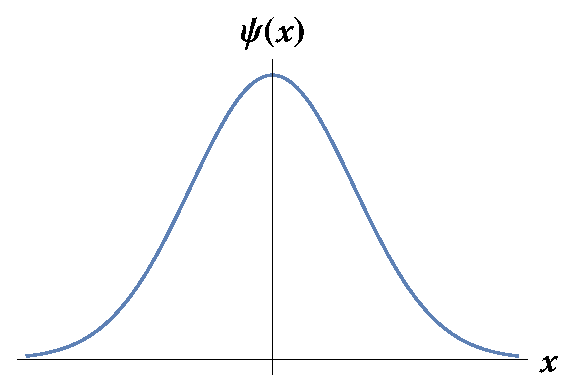
\includegraphics[scale=0.7]{fig/2-3-a.eps}
        }
        \subfigure[$n=2$]{
            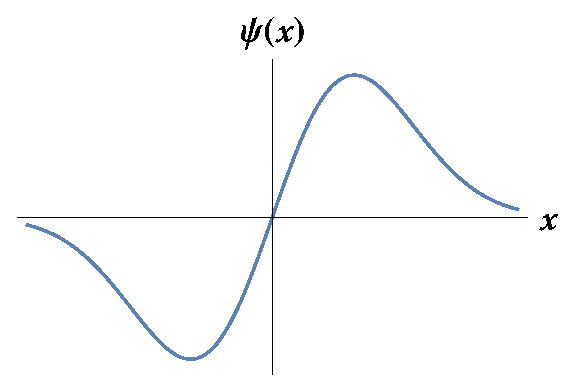
\includegraphics[scale=0.7]{fig/2-3-b.eps}
        }   
        \subfigure[$n=3$]{
            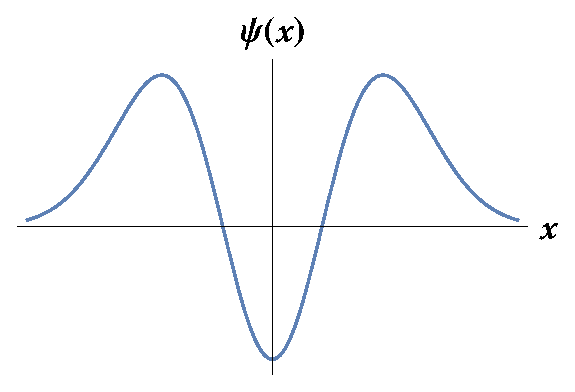
\includegraphics[scale=0.7]{fig/2-3-c.eps}
        }   
        \caption{可以看到, 图像之间的递推联系还是满足前面的规则的}
    \end{figure}

    \subsection{分析方法}
    \begin{define}{两个无量纲数}
        \begin{center}
            \begin{math}
            \displaystyle
            \xi = \sqrt{\frac{m\omega}{\hbar}}x \qquad\qquad K=\frac{2E}{\omega\hbar}
            \end{math}
        \end{center}
    \end{define}
    重写方程为:
    \begin{lequation}
        \label{rewrite}
        \frac{d^2\psi}{d\xi^2}=(\xi^2-K)\psi
    \end{lequation}
    \begin{thinknote}
        你可能对这个形式的得到有所疑问, 实际上, 这就是一个求导的链式法则的问题, 注意, 换元前的方程$\frac{d\psi}{dx}$表示把$\psi$写成$f(x)$后再求导, 而
        换元后的方程中$\frac{d\psi}{d\xi}$表示将$\psi$表示为$\phi(\xi)$后再进行求导。而$\xi=\varphi(x)$, 使用链式法则便可以理解这里的换元了。
    \end{thinknote}
    使用幂级数方法求解的第一步就是去求其\uwave{渐进解}, 也就是说去观察$\xi \to \pm\infty$的时候方程的行为。这个方程在$\xi\gg K$时
    $$\frac{d^2\psi}{d\xi^2}\approx\xi^2\psi$$这个方程的通解形式是$$\psi\approx Ae^{-\xi^2/2}+Be^{\xi^2/2}$$显然$B\neq 0$时波函数不能进行归一化, 所
    以, 方程\ref{rewrite}的解的形式应该是$\psi = h(\xi)e^{-\xi^2/2}$, 代入后有$$\frac{d^2h}{d\xi^2}-2\xi\frac{dh}{d\xi}+(K-1)h=0$$这是一个二阶方程
    但是是变系数, 所以也很难求解, 只能考虑使用幂级数解法, 两边进行Taylor展开后解得$$h(\xi)=\sum_{j=0}^\infty a_j\xi^j,\qquad a_{j+2}=\frac{2j+1-K}{(j+1)(j+2)}a_j$$
    我们只要确定$a_0$和$a_1$也就可以确定解, 二阶方程刚好两个待定系数, 但是我们只有波函数归一化这一个方程似乎无法去完整的确定两个待定系数。这里的原因是能量
    的量子化取值, 导致了最后方程只会含有一个待定系数。

    我们可以证明, $h(\xi)$只能在某些特定的情况下在$\xi \to \pm \infty$时收敛, 这也就决定了\textbf{$K$的取值是量子化的}。事实上, 收敛的充要条件是, 上面的数列$\{a_j\}$
    会终止于$0$。
    \begin{proposition}{$a_j$会终止于$0$}
        \begin{center}
            \begin{math}
            \displaystyle
            K=2n+1,\quad (n=0,1,2,\ldots)
            \end{math}
        \end{center}
        如果$n$是奇数, 那么$a_{2n+1}$会终止于$0$, 但是$a_0=0$也就是说必须有$a_{2n}\equiv 0$, $n$为偶数时类似
    \end{proposition}
    这样方程最终得到的解就只会有一个待定系数了, 而且由递推公式得知是正比于$a_0$或$a_1$的, 再利用归一化条件便可以得到解
    \begin{define}{厄米多项式}
        把$h(\xi)$的$a_0$或者$a_1$因子去掉并且乘上一个数将最高次项前面的因子化为$2^n$, 得到的多项式为\textbf{厄米多项式}, 记作$H_n(\xi)$\\
        例如:$h_2(\xi)=a_0(1-2\xi^2)=-\frac{1}{2}a_0(4\xi^2-2)$则$H_2(\xi)=4\xi^2-2$
    \end{define}
    我们不加证明地列出波函数归一化后的解与厄米多项式之间的关系\footnote{前面因子的相位按照惯例按最简单的取}:
    \begin{lequation}
        \boxed{
            \psi(x)=\left(\frac{m\omega}{\pi\hbar}\right)^{\frac{1}{4}}\frac{1}{\sqrt{2^nn!}}H_n(\xi)e^{-\xi^2/2}
        }
    \end{lequation}
    \begin{theorem}{$H_n(\xi)$的诸多性质}
        \begin{itemize}
            \item 
                \begin{math}
                    \displaystyle
                    H_n(\xi)=(-1)^ne^{\xi^2}\left(\frac{d}{d\xi}\right)^ne^{-\xi^2}
                \end{math}
            \item 
                \begin{math}
                    \displaystyle
                    H_{n+1}(\xi)=2\xi H_n(\xi)-2nH_{n-1}(\xi)
                \end{math}
            \item 
                \begin{math}
                    \displaystyle
                    \frac{d H_n}{d\xi}=2n H_{n-1}(\xi)
                \end{math}
            \item 
                \begin{math}
                    \displaystyle
                    e^{-z^2+2z\xi}=\sum_{n=0}^{\infty}\frac{z^n}{n!}H_n(\xi)\quad\text{(generate function)}
                \end{math}
        \end{itemize}
    \end{theorem}
    量子效应下, 谐振子的行为和经典力学非常不同, 不再有\uwave{振幅}这一概念, 粒子可以在无穷远处被发现, 不违背能量守恒定律正是因为量子力学中, 我们只谈系综的
    力学量的平均值, 不再对于某个粒子有诸如动能这些的定义了, 我们只讲系综的平均效应, 只谈概率, 不谈确定性。
    \section{自由粒子}
    自由粒子情况下即$V \equiv 0$, 不难发现定态薛定谔方程和无限深势阱的形式是一样的, 即$$\frac{d^2\psi}{dx^2}=-k^2\psi$$解的形式为$$Ae^{ikx}+Be^{-ikx}$$
    注意, \uwave{我们不再有边界条件去直接确定$A$和$B$的值}, \textbf{这个时候定态解的能量的取值并不是离散的!可以取到任何大于$0$的值!}其实本身量子力学就是不排斥
    连续性的, 离散可以有很多种, 不一定就表明某个量一定是离散取值。

    考虑wiggle-function后写成下面的形式\footnote{这里$\psi_k$无法进行归一化, 我们这里添上系数${\raise0.5ex\hbox{$\scriptstyle 1$}\kern-0.1em/\kern-0.15em
    \lower0.25ex\hbox{$\scriptstyle {\sqrt {2\pi } }$}}$是狄拉克意义下的正交归一化的考虑。}:
    \begin{lequation}
        \boxed{
            \Psi_k(x,t)=Ae^{i\left(kx-\frac{k^2\hbar t}{2m}\right)}, \psi_k(x)=\frac{1}{\sqrt{2\pi}}e^{ikx}
        }
    \end{lequation}
    
    \begin{thinknote}
        实际上我们更常见的写法是用:
        \[\psi_p(x)=\frac{1}{\sqrt{2\pi\hbar}}e^{i\frac{p}{\hbar}x}\]
        作为自由粒子体系的能量表象, 这和动量表象表达式相同。详见下一章讨论。
    \end{thinknote}
    
    考虑到最后反正要对解进行线性叠加, 而两项仅仅只在$e$指数上面差了一个负号, 所以我们将负号纳入$k$后得到:
    $$k\overset{def}{=}\pm\frac{\sqrt{2mE}}{\hbar}$$观察到每一项就代表一个\uwave{行波}, $k>0$的时候正向传播(向右), 反之负向传播, 不再是前面势阱模型里面的
    驻波。
    \begin{thinknote}
        对于某个确定的振幅对应了一个$x$, 也就是说概率波上面的某一个确定的点, 其$x$和$t$之间满足$x\pm vt=\text{const}$的演化关系, 也即$x=\mp v +\text{const}$。所以可以认为概率
        波上的每个点都以$v$的速度在\uwave{平移运动}, 也很容易根据速度前的正负号确定是左行波还是右行波了。顺带一提, 这种形式下的行波, 模长平方(概率密度)与位置
        无关(不同位置找到粒子概率都一样), 都等于指数项前面振幅的平方, 这也是后面$\delta$势阱散射态求透射系数的基础。
    \end{thinknote}
    
    与经典力学中的波动方程相对应, 前面讲过$k$可以理解为角波数, 那么波速$v=\frac{|k|\hbar}{2m}=\sqrt{\frac{E}{2m}}$, 角频率$\omega=\frac{k^2\hbar}{2m}$, 过会我们会再回到波速的问题上来, 目前
    来看似乎有自由粒子速度$v_p=\sqrt{\frac{2E}{m}}=2v_{wave}$。

    自由粒子的波函数的定态解与前面两个模型最大的不同就是\textbf{它是无法归一化的}。所以现在我们求出来的定态解完全只是数学上的一个过程\footnote{虽然不存在这样一个定态, 但是我们前面介绍的解薛定谔方程的一般手段仍旧不变, 只是这些“定态”不可归一化且是连续谱}, 没有实际的物理意义
    不存在一个状态, 其中自由粒子属于能量始终不变的定态(无论如何测量都是一个值)。但是没事, 虽然不存在定态, 但是我们还是可以使用定态解的线性组合来构造符合初值的
    解\footnote{这些合成的解沿用波动学的观点, 称为\uwave{波包}, 是可归一化的}, 这些“定态”解也是归一化和完备的。

    我们仍旧对定态解进行线性叠加, 注意是对定态解叠加, 也就是对定态解的波函数进行叠加不是$\psi$而是$\Psi$, 所以不要忘记了每个$\psi$后面的关于时间的指数项。
    \begin{lequation}
        \label{2.26}
        \boxed{
            \Psi=\int_{-\infty}^{\infty}\phi(k)\psi_ke^{-\frac{ik^2\hbar}{2m}t}dk=\frac{1}{\sqrt{2\pi}}\int_{-\infty}^{\infty}\phi(k)e^{i\left(kx-\frac{k^2\hbar}{2m}t\right)}dk  
        }
    \end{lequation}
    和\ref{find_c}对比一下就会发现, $\phi(k)$取代了$c_n$, 这一点很好理解, 因为$\phi_k(x)$变成了一个关于$k$的连续函数, 而数列我们也通常称为\uwave{整标函数}, 所
    以, 前面变成连续函数来加权, 求和也变成了积分。

    初始值还是在$t=0$处给定\footnote{若不是, 你对$t$进行一个换元平移一下计时零点即可}, 那么可以得到:
    \begin{lequation}
        \Psi(x,0)=\frac{1}{\sqrt{2\pi}}\int_{-\infty}^{\infty}\phi(k)e^{ikx}dk  
    \end{lequation}
    数学上$\Psi$就是对$\phi$的\uwave{傅里叶逆变换}, 下面的定理可以很方便的求出$\phi(k)$。
    \begin{theorem}{Plancherel's theorem}
        \begin{center}
            \begin{math}
                \displaystyle
                f(x)=\frac{1}{\sqrt{2\pi}} \int\limits_{-\infty}^{\infty}F(k)e^{ikx}dk\Longleftrightarrow F(k)=\frac{1}{\sqrt{2\pi}} \int\limits_{-\infty}^{\infty}f(x)e^{-ikx}dx
            \end{math}
        \end{center}
    \end{theorem}

    其中$F(x)$表示$f(x)$的傅里叶变换, 反之即为逆变换。
    \begin{lequation}
        \boxed{
            \phi(k)=\frac{1}{\sqrt{2\pi}} \int _{-\infty}^{\infty}\Psi(x,0)e^{-ikx}dx
        }
    \end{lequation}
    
    遗憾的是, 很多函数都只能写出积分后进行数值模拟, 无法用基本初等函数表示。
    \begin{define}{群速度和相速度}
        \begin{itemize}
            \item \textbf{群速度}:波包的移动速度
            \item \textbf{相速度}:波包里面有很多小峰, 这些小峰的移动速度便是相速度, 可以理解为一个在波上的质点跟随波的平移速度
        \end{itemize}
    \end{define}
    \begin{center}
       \animategraphics[scale=0.8,autoplay=True,loop]{24}{videos/wave_group/wave_group-}{0}{250} 
    \end{center}
    \begin{center}
        上面的动画中, {\color{red}红色}表示相速度, {\color{green}绿色}表示群速度
    \end{center}
    
    关于群速度和相速度的讨论应该是波动学的内容, 这里我们不想讨论过多, 只是先说明两个速度的计算公式, 在波包很明显也就是有很好的群速度的定义的时候, 单单从
    自由粒子的波动方程可以推出下面这一点。
    \begin{theorem}{群速度和相速度的计算}
        \begin{lequation}
            \boxed{
               v_g=\frac{d\omega}{dk}\qquad\qquad v_p=\frac{\omega}{k} 
            }
        \end{lequation}
    \end{theorem}
    其中, 波包是由一系列定态解叠加而成的, 具有下面的形式(对比\ref{2.26}):
    $$\Psi=\frac{1}{\sqrt{2\pi}}\int_{-\infty}^{\infty}\phi(k)e^{i\left(kx-\omega t\right)}dk,\quad \omega=\frac{k^2\hbar}{2m}$$
    正是由于多列行波的叠加才形成了波包, 而每个分量(行波)中的频率又是和$k$相关的, 这样就会导致群速度不等于相速度, 这时我们称之为\textbf{色散}, 自由粒子的
    波函数恰好就是多列行波的叠加, $\omega$是关于$k$的二次式, 那么, 代表粒子的群速度是代表行波前进的相速度的两倍这一论断就不难看出了。
    \section{\texorpdfstring{$\delta$}.函数势阱}
    \subsection{束缚态和散射态}
    最好引入束缚态和散射态的方法是使用经典类比, 我们前面提到的谐振子和无限深势阱都是束缚态, 他们每个定态解是可归一化的, 而且是分立谱, 粒子的行为像驻波一
    般, 会因为某些特定的边界条件使得波函数被限制在一个局域内。但是后面讲的自由粒子是连续谱, 不存在定态, 定态解不可归一化, 它的行为更像是一种行波, 可以自
    由延伸到无穷远处, 但是由定态解的线性组合构成的波包是可以归一化的, 这也就意味着, 一旦我们讨论的是自由粒子这种散射态, 他一定是很多种
    定态能量的叠加态, 不可能是测量后只会出现一种能量的某个定态, 一定是很多很多定态的组合, 因为对于散射态定态解是没有物理意义的, 这一点我们后面会再次提到。

    从经典力学来看, 由于物体的动能始终是一个定值, 所以在势能图上, 粒子永远不可能达到势能大于粒子总能量的地方(能量守恒), 从图上来看就是粒子被限制在两个点
    之间来回折返(\ref{turning_point}), 除非物体的能量大于势能的最大值, 这样粒子就会越过“山峰”, 不断前进。
    \begin{figure}[htbp]
        \centering
        \label{turning_point}
        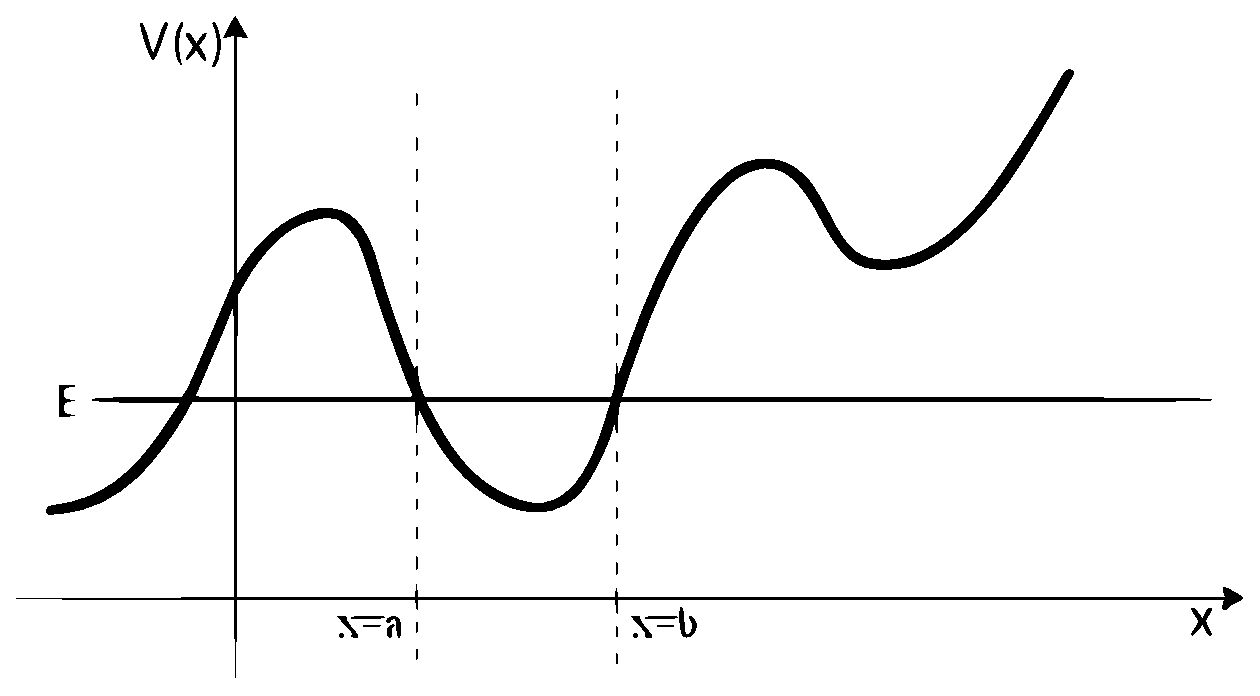
\includegraphics[scale=0.5]{fig/2-5-1.eps}
        \caption{经典力学中, 粒子会被“困在”$x=a$和$x=b$之间}
    \end{figure}
    还是以上面的图像为例, 在经典力学看来(如果初始位置在$ab$之间的话), 这个图像会产生一个束缚态, 在量子力学中, 马上你将会看到, 由于所谓的\textbf{量子隧穿效应}
    , 任何有限高的势能都不能阻挡粒子, 粒子完全可以越过最高点大于其总能量的“山峰”。所以上面的图像对于量子理论来说也是一个散射态, 只有像前面所说的无限深势阱和
    谐振子, 才会导致粒子的束缚态的产生。
    \begin{theorem}{束缚态和散射态的判定准则}
        \begin{center}
            \begin{math}
                \displaystyle
                \begin{cases}
                    E>V(+\infty) \vee E>V(-\infty) \Rightarrow \text{Bound State}\\
                    E<V(+\infty) \wedge E<V(-\infty) \Rightarrow \text{Scattering State}
                \end{cases}
            \end{math}
        \end{center}
        一般情况下, $V(x)$会在$x\to\pm\infty$时趋近于$0$(谐振子和无限深势阱就是特例), 这个时候可以再次简化判定准则为:
        \begin{center}
            \begin{math}
                \displaystyle
                \begin{cases}
                    E>0 \Rightarrow \text{Bound State}\\
                    E<0 \Rightarrow \text{Scattering State}
                \end{cases}
            \end{math}
        \end{center}
    \end{theorem}
    注意, 我们前面在求解薛定谔方程时, 都说过$E>V_{min}$, 很遗憾, 这个条件在散射态时, 不起作用, 因为散射态我们并不严格要求定态解一定是可归一化的, 所以这
    个条件只能对于束缚态使用, 前面我们对谐振子和无限深势阱使用这个条件是完全正确的, 因为无论$E$是大于$0$还是小于$0$, 这两个势阱产生的都是束缚态, 那么束缚
    态的定态解必须是可归一化的, 这也就间接要求了$E$的非负性。事实上, 你如果在$E<0$的假定下求解这两种模型的解, 你会发现无论是定态还是线性组合后的解都是不可归一化的
    , 没有实在的物理意义。 在这个时候我们就说$E>0$的解已经构成了一个\uwave{完备集}, 初始的波函数一定是可以归一化的, 也一定是可以由对应的定态解组合而成, 然而
    $E<0$的解都不可以归一化, 所以这两种势能模型中仅当粒子$E>0$时有物理意义, 这一点实际上根据经典力学我们可以很容易类比得出。

    \subsection{\texorpdfstring{$\delta$}d函数势阱}
    注意这里我们讨论的是\uwave{势阱}, 主要是为了和后面的\uwave{势垒}区分, 你可以将势阱想象成一口井, 但势垒是一座山。
    \subsubsection*{狄拉克$\delta$函数}
    这个函数的定义你可以立即为将克罗内克符号扩充为一个连续函数, 也可以理解为是以个函数序列的极限。
    \begin{define}{$\delta$ function}
        \begin{center}
            \begin{math}
                \displaystyle
                \delta(x)\equiv
                \begin{cases}
                    0, x\neq 0\\
                    +\infty,x=0
                \end{cases},\text{but}\int_{-\infty}^{+\infty}\delta(x) dx=\int_{0^-}^{0^+}\delta(x) dx=1
            \end{math}
        \end{center}
    \end{define}
    \begin{proposition}{$\delta$函数的提取性质}
        \begin{itemize}
            \item $f(x)\delta(x-a)=f(a)$
            \item $\int_{-\infty}^{\infty}f(x)\delta(x-a)=f(a)$
        \end{itemize}
    \end{proposition}
    我们现在考虑的势阱形式是$V(x)=-\alpha\delta(x),\alpha>0$。显然, $E>0$时是散射态, $E<0$时是束缚态\footnote{考虑束缚态时, 除了根据判据, 你还要
    观察下, 在这个能量条件下, 定态解是不是平方可积的, 满足束缚态的定义, 在这里由于$V_{min}\to -\infty$, 所以恒有$E>V_{min}$, 粗略来看束缚态是可以在这个
    能量条件下给出的, 后面的势垒就是个反例。}。
    \subsubsection*{束缚态($E<0$)}
    定态薛定谔方程:
    \begin{center}
        \begin{math}
            \displaystyle
            -\frac{\hbar^2}{2m}\frac{d^2\psi}{dx^2}-\alpha\delta(x)\psi=E\psi
        \end{math}
    \end{center}
    定义$\kappa\equiv\frac{\sqrt{-2mE}}{\hbar}$, 这个解应该是一个分段函数形式, 分段求解首先考虑$x<0$, 方程可以写成:
    $$\frac{d^2\psi}{dx^2}=\kappa^2\psi$$方程的通解具有形式$\psi(x)=Ae^{\kappa x}+Be^{-\kappa x}$, 实际上对于波函数, 我们有下面的必要边界条件\footnote{实际上是量子力学几条基本原理之一}:
    \begin{proposition}{$\psi$标准条件}
        \begin{itemize}
            \item \textbf{连续性}: $\psi(x)$是一个连续函数
            \item \textbf{一阶导数连续性}: 除了$\delta(x)$这样的奇异函数$\frac{d\psi}{dx}$具有连续性
            \item \textbf{单值性}: 显然一个点只能对应一个概率密度
            \item \textbf{有界性}: $x\to\pm\infty$时, $\psi(x)$不能趋近于无穷大
            \item \textbf{归一化条件}: 当然现在我们\uwave{只能对束缚态这么做了}, 可以用这个定出每个定态前的系数
        \end{itemize}
    \end{proposition}
    利用有界性我们直接推出$A=0$, $x>0$时, 同样分析可以得出$\psi(x)=Fe^{\kappa x}+Ge^{-\kappa x}$, 其中$F=0$。另外, 利用在$x=0$处的连续性可以得到$B=G$
    , 但是在$x=0$处一阶导\uwave{并不连续}, 我们对定态方程两边积分可以得到$$\frac{\hbar^2}{2m}\left[\psi'_+(0)-\psi'_-(0)\right]+\alpha\psi(0)=0$$
    然后再代入$\psi'_+(0)-\psi'_-(0)=-2\kappa B$并进行归一化后不难得到
    \begin{lequation}
        \boxed{
            \psi(x)=\frac{\sqrt{m\alpha}}{\hbar}e^{-m\alpha\left|x\right|/\hbar^2}, \qquad E=-\frac{m\alpha^2}{2\hbar^2}
        }
    \end{lequation}
    
    通常的束缚态都有无穷多个定态, 但是这个问题却出奇的单调, 只有一个定态, 只有一种能量的可取值。
    \begin{figure}[htbp]
        \centering
        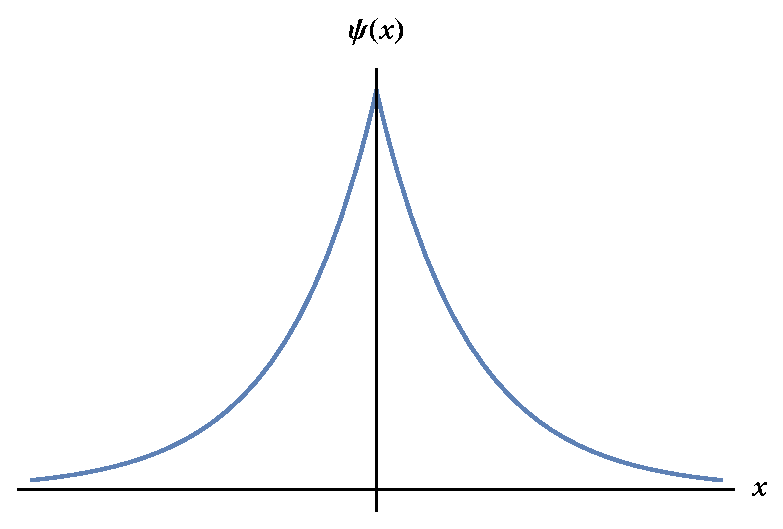
\includegraphics[scale=0.5]{fig/2-5-2.eps}
        \caption{这是束缚态$\psi$图像, 不是概率密度曲线}
    \end{figure}
    \subsubsection*{散射态($E>0$)}
    散射态比较难以处理, 我们还是分段考虑我们可以得到下面的解:
    \begin{center}
        \begin{math}
            \displaystyle
            \psi(x)=
            \begin{cases}
                Ae^{ikx}+Be^{-ikx},x<0\\
                Fe^{ikx}+Ge^{-ikx},x<0
            \end{cases}
            ,k=\frac{\sqrt{2mE}}{\hbar}
        \end{math}
    \end{center}
    遗憾的是, 这次我们不能通过有界性指出哪一项前面的系数一定为$0$了, 散射态最明显的性质就是\textbf{$\psi$在无穷远处不会趋近于$0$, 也就是说不像束缚态
    的驻波性质一般被局限在某个范围内}, 它更像是在描述一个粒子从无穷远处来, 过散射中心后到无穷远处去, 所以被称作\uwave{散射态}。

    不过好在波函数的连续性还在, 我们还是可以通过对方程两边积分得到导数的跃变关系, 同束缚态一样, 我们得到:
    $$A+B=F+G$$ $$F-G=(1+2i\beta)A-(1-2i\beta)B$$其中$\beta\equiv\frac{m\alpha}{k\hbar^2}$。这是一个不定方程, 我们还缺少初始波函数条件, 虽然这样的定态是
    不存在的, 只有它们合成的波包才有意义, 但是不妨碍我们去考察一下这个解背后蕴含的思想, 实际上和光学上的反射和透射非常相似。
    
    之前我们求解自由粒子的波函数的时候发现, 考虑了含时指数因子后$$\Psi_k(x,t)=A\exp\left[i\left(kx-\frac{k^2\hbar}{2m}t\right)\right]$$在$k>0$时表示
    向右传播的行波, 反之表示向左传播的行波。结合这个问题, 考虑的解的区间, 这个解可以看作是
    \begin{itemize}
        \item $x<0$,$-\infty\to0$的振幅为$A$的波和$0\to-\infty$的振幅为$B$的波;
        \item $x>0$,$+\infty\to0$的振幅为$G$的波和$0\to+\infty$的振幅为$F$的波。
    \end{itemize}
    我们考虑比较简单的情况即$G=0$, 也就是说粒子从左边入射, 然后在$x=0$处就如有一个介质一般, 粒子的入射波一部分被反射($B$)一部分透射($F$)
    \begin{lequation}
        F=\frac{1}{1-i\beta}A,\quad B=\frac{i\beta}{1-i\beta}A
    \end{lequation}
    我们还可以同光学一样, 讨论相对于原先的入射波, 透射波和反射波损失了多少, 即透射系数($T$)和反射系数($R$):
    \begin{lequation}
        \begin{aligned}
            &R\equiv\frac{|B|^2}{|A|^2}=\frac{\beta^2}{1+\beta^2}\\
            &T\equiv\frac{|F|^2}{|A|^2}=\frac{1}{1+\beta^2}\\
            &R+T=1
        \end{aligned}
    \end{lequation}

    我们再将其写成能量的关系式:
    \begin{lequation}
        \boxed{
            R=\frac{1}{1+\left(2\hbar^2E/m\alpha^2\right)}, T=\frac{1}{1+\left(m\alpha^2/2\hbar^2E\right)}
        }
    \end{lequation}

    能量越高透射波的振幅越大, 也就是说粒子\uwave{穿过}势阱的可能性越高, 这显然是与常识相符的。

    当然, 由于定态解合成的波包才是真正有物理意义的解, 所以我们推出来的$R$和$T$应当理解成粒子的能量在某一个很小的范围的时候的近似值\footnote{前面提到过需要多个态叠加
    才有物理意义, 这也就意味着粒子测量时的能量一定是在某个连续的范围内, 散射态的能量本征值是连续谱。}
    \subsubsection*{$\delta$函数势垒}
    形式上来看势垒的解形式上应该和上面讨论的势阱的散射态相同, 只是$\alpha$的符号刚好相反。但是透射系数和反射系数是不变的。
    \begin{thinknote}
        注意, 这个时候是不存在束缚态的, 你可以这么想, 如果存在束缚态, 那么束缚态的定态一定可归一化, 那么$E>V_{min}=0$, 但是根据判定条件, 或者解方程可以明显
        的发现$E>0$的时候是一个散射态, 就如谐振子和自由粒子一样, $E>0$的解构成了一个完备集。
    \end{thinknote}
    那么既然透射系数不一定为$0$, 也就是说, 和经典情况不同, 经典力学中, 粒子不可能穿过$\delta$势垒, 但是量子散射效应下, 粒子完全有概率穿过势垒, 而且与其
    携带的能量正相关, 这种现象称之为\textbf{量子隧穿效应}, 在电子显微镜及其它很多领域中有广泛的应用。
    \subsubsection*{$\delta$函数势阱束缚态计算}
    我们之前讲的计算方法就是利用连续性和薛定谔方程两端积分, 这对于只有一个$\delta$函数的势阱很实用, 但是$\delta$函数数目较多时, 由于还要分段求解方程, 计算就显得比较繁琐了, 下面介绍一种
    利用傅里叶变换快速计算的方法\footnote{cf.顾樵, 量子力学, vol.1, P140-144}。

    傅里叶变换使用如下定义方法:
    \begin{equation}
        \label{傅里叶变换}
        \begin{aligned}
        \mathscr{F}[f(t)] &=F(\omega)=\int_{-\infty}^{+\infty} f(t) e^{-i \omega t} d t \\
        \mathscr{F}^{-1}[F(\omega)] &=f(t)=\frac{1}{2 \pi} \int_{-\infty}^{+\infty} F(\omega) e^{i \omega t} d \omega
        \end{aligned}
    \end{equation}
    \begin{proposition}{傅里叶变换常用性质}
        \begin{itemize}
            \item \textbf{线性性}\footnote{使用$\mathscr{F}$表示变换, 大写字母表示变换后相应的函数}:$$
            \begin{gathered}
            \mathscr{F}[\alpha f(t)+\beta g(t)]=\alpha F(\omega)+\beta G(\omega) \\
            \mathscr{F}^{-1}[\alpha F(\omega)+\beta G(\omega)]=\alpha f(t)+\beta g(t)
            \end{gathered}$$
            \item \textbf{位移性}:$$
            \begin{gathered}
            \mathscr{F}\left[f\left(t-t_{0}\right)\right]=e^{-i \omega t_{0}} F(\omega) \\
            \mathscr{F}^{-1}\left[F\left(\omega-\omega_{0}\right)\right]=e^{i \omega_{0} t} f(t)
            \end{gathered}
            $$
            \item \textbf{放缩性}:$$
            \mathscr{F}[f(a t)]=\frac{1}{|a|} F\left(\frac{\omega}{a}\right)
            $$
            \item \textbf{对称性}:$$
            \mathscr{F}[F(t)]=2 \pi f(-\omega)
            $$
            \item \textbf{微分关系}:$$
            \begin{gathered}
            \mathscr{F}\left[\frac{d^{n} f(t)}{d t^{n}}\right]=(i \omega)^{n} F(\omega) \\
            \mathscr{F}^{-1}\left[\frac{d^{n} F(\omega)}{d \omega^{n}}\right]=(-i t)^{n} f(t)
            \end{gathered}$$
            \item \textbf{积分关系}:$$\mathscr{F}\left[\int f(t)dt\right]=\frac{1}{i\omega}F(\omega)$$
            \item \textbf{帕萨瓦尔定理}:$$
            \int_{-\infty}^{+\infty} f(t) g^*(t) d t=\frac{1}{2 \pi} \int_{-\infty}^{+\infty} F(\omega) G^*(\omega) d \omega
            $$
            \item \textbf{时域卷积定理}:$$
            \mathscr{F}[f(t) * g(t)]=F(\omega) G(\omega)
            $$
            \item \textbf{频域卷积定理}:$$
            \mathscr{F}[f(t) g(t)]=\frac{1}{2 \pi} F(\omega) * G(\omega)
            $$
            \item \textbf{与$\delta$函数关系}:$$\delta(x)=\mathscr{F}^{-1}[1](x)$$
        \end{itemize}
    \end{proposition}

    我们下面以双$\delta$势阱为例来讲解这种方法。
    \begin{define}{双$\delta$势阱}
        \begin{equation}
            V(x)=-\alpha\left[\delta(x-a)+\delta(x+a)\right]
        \end{equation}
    \end{define}
    定态薛定谔方程写为:
    \begin{equation}
        -\frac{\hbar^2}{2m}\frac{d^2\psi}{dx^2}-\alpha\left[\delta(x-a)+\delta(x+a)\right]\psi=E\psi
    \end{equation}
    方程两边进行傅里叶变换(\ref{傅里叶变换}), $k$的定义同前, 有:
    \begin{equation}
        \begin{aligned}
        -\omega^2\mathscr{P}(\omega)-k^2\mathscr{P}(\omega)&=-\frac{2m\alpha}{\hbar^2}\int_{-\infty}^{\infty}\left[\delta(x-a)+\delta(x+a)\right]\psi(x)e^{-i\omega x}dx\\
        &=-\frac{2m\alpha}{\hbar^2}\left(e^{i\omega a}\psi(-a)+e^{-i\omega a}\psi(a)\right)
        \end{aligned}
    \end{equation}
    其中$\mathscr{F}\left[\psi(x)\right](\omega)\equiv\mathscr{P}(\omega)$, 解得:
    \begin{equation}
        \mathscr{P}(\omega)=\frac{2m\alpha}{\left(k^2+\omega^2\right)\hbar^2}\left(e^{i\omega a}\psi(-a)+e^{-i\omega a}\psi(a)\right)
    \end{equation}
    再进行傅里叶逆变换得到:
    \begin{equation}
        \psi(x)= \frac{m\alpha}{k\hbar^2}\left[\psi(a)e^{-k|x-a|}+\psi(-a)e^{-k|x+a|}\right]
    \end{equation}
    上式中, 我们取$x=-a$和$x=a$得到:
    \begin{equation}
        \begin{pmatrix}
            \frac{m\alpha}{k\hbar^2}-1&\frac{m\alpha}{k\hbar^2}e^{-2ka}\\
            \frac{m\alpha}{k\hbar^2}e^{-2ka}&\frac{m\alpha}{k\hbar^2}-1
        \end{pmatrix}
        \begin{pmatrix}
            \psi(a)\\
            \psi(-a)
        \end{pmatrix}
        =\begin{pmatrix}
            0\\0
        \end{pmatrix}
    \end{equation}
    这个方程显然必须要有非零解, 倘若只有平凡解, 则$\psi(x)\equiv0$, 显然不能归一化。对于非零解, 最终定态解的系数由归一化条件确定。
    \begin{equation}
        \Delta=\begin{vmatrix}
            \frac{m\alpha}{k\hbar^2}-1&\frac{m\alpha}{k\hbar^2}e^{-2ka}\\
            \frac{m\alpha}{k\hbar^2}e^{-2ka}&\frac{m\alpha}{k\hbar^2}-1
        \end{vmatrix}=0
        \Rightarrow e^{-2ka}=\pm\left(1-\frac{k\hbar^2}{m\alpha}\right)
    \end{equation}
    上式给出的是一个超越方程, 我们对它进行如下变形:
    \begin{equation}
        \left.\begin{matrix} 
           X\equiv 2ka=\frac{2a\sqrt{-2mE}}{\hbar}\\
            \sigma\equiv\frac{\hbar^2}{2ma\alpha}\\
            y^\pm(x) \equiv 1-\sigma X
          \end{matrix}\right\}\Rightarrow Y(X)=y^\pm(x)
    \end{equation}
    绘图后可以发现$\sigma<1$时图像有两个交点, $\sigma\geq 1$时图像只有一个交点, 而交点的个数就代表着能量的可取值, 一个交点对应了一个束缚态。
    \begin{center}  
        \animategraphics[scale=0.75,autoplay=True,loop]{8}{videos/equation_insection/equation_insection-}{0}{59}
    \end{center}
    \newpage
    \section{有限深势阱}
    \begin{define}{有限深势阱}
        \begin{center}
            \begin{math}
                \displaystyle
                V(x)=\begin{cases}
                    -V_0,\quad &-a\leq x \leq a\\
                    0, &|x|>a
                \end{cases}
            \end{math}
        \end{center}
    \end{define}
    对于束缚态, 定义$k\equiv\frac{\sqrt{-2mE}}{\hbar}$, 对于散射态定义$k\equiv\frac{\sqrt{2mE}}{\hbar}$, 无论散射态还是束缚态, 统一定义
    $l=\frac{\sqrt{2m\left(E+V_0\right)}}{\hbar}$。
    \subsection*{束缚态($E<0$)}
    \subsubsection*{(\romannumeral1)$x<a$}
    这个范围内$V=0$, 利用$\psi(-\infty)=0$的边界条件可以得到解为:$$\psi(x)=Ae^{kx}$$
    \subsubsection*{(\romannumeral2)$-a\leq x\leq a$}
    这个范围内$V=-V_0$, 通解的指数形式为$Ce^{ilx}+De^{-ilx}$, 这种形式我们称之为\textbf{行波形式}, 主要是散射态用的多。还可以利用Euler公式写成三角
    形式为$C\cos (lx)+D\cos (lx)$, 这种我们一般称为\textbf{驻波形式解}。这两种表达方式是完全等价的, 其中两个任意常数在复数域中取值在这里我们采用第二种
    驻波形式, 后面的数学处理更加简便。我们有:$$\psi(x)=C\cos (lx)+D\cos (lx)$$
    \subsubsection*{(\romannumeral3)$x>a$}
    和第一个范围形式一样, 为:$$\psi(x)=Fe^{-kx}$$
    \subsubsection*{边界条件}
    利用$\psi(x)$和$\psi\prime(x)$的连续性可以列出四个方程, 再利用归一化条件便可以完全定下五个参数。这里我们使用了一阶导的连续性, 实际上, 只要势能的性质
    并不是像$\delta$函数这么坏, 这个条件都是成立的, 不成立时我们可以得到两侧导数之间的关系。

    其实, 我们可以使用对称性进一步简化我们的运算\footnote{如果没有想到对称性, 直接根据方程组有非零解, 系数行列式为0, 也可以计算出能级, 只是最后波函数的形式有点不同。}, 在束缚态的求解中, 下面的陈述十分有效:
    \begin{proposition}{定态波函数的对称性}
        如果所给势能$V(x)$是一个\textbf{偶函数}, 那么$\psi(x)$\textbf{总可以取作偶函数或者奇函数}\footnote{注意这里是\uwave{取作},意思是用奇函数和偶函数作为基底是完全等价的, 不是说$\psi$一定有奇偶性}, 分奇偶讨论后根据条件取舍就可以得到全部的解。
    \end{proposition}
    上面的定理告诉我们可以只关心那些有对称性的解, 计算结果等价。下面分类求解。
    
    首先讨论偶函数情况, 我们事先将$\psi(x)$在势阱内部的形式写成了驻波解形式, 这样我们就很容易根据对称性进一步得出$D=0$, 事实上, 实际问题求解中到底选择
    行波形式还是驻波形式就是要尽可能让其中的一个待定系数为$0$, 比如$\delta$势阱散射态中我们取行波形式, 一是为了突出问题的物理内涵, 二是可以直接去掉另一个
    方向入射的波。我们还得到了$A=F$这个关系。

    利用边界条件和方程解算后可以得到:$$k=l\tan(al)$$我们再一次得到了能量取值应满足的条件, 这又是一个超越方程需要数值求解。我们不去具体计算能量, 我们通过这个式子将波函数进行
    归一化处理, 仍旧最简单的选取系数的相位, 可以得到:
    \begin{equation}
        \psi(x)=\begin{cases}
            \frac{e^{ka}\cos(la)}{\sqrt{a+1/k}}e^{kx},&x<-a\\
            \frac{1}{\sqrt{a+1/k}}\cos(lx),&-a\leq x\leq 0\\
        \end{cases}
    \end{equation}
    利用$\psi(x)$是偶函数可以得到另一边的解。

    同理, 对于奇函数情况, 我们可以得到$A=-F$, $C=0$。解得:$$k=-l\cot (la)$$归一化得到:
    \begin{equation}
        \psi(x)=\begin{cases}
            \frac{e^{ka}\cos(la)}{\sqrt{a+2\cos^2(la)/k}}e^{kx},&x<-a\\
            \frac{1}{\sqrt{a+2\cos^2(la)/k}}\sin(lx),&-a\leq x\leq 0\\
        \end{cases}
    \end{equation}
    利用$\psi(x)$是奇函数可以得到另一边的解。

    值得注意的是, 上面的解在$V_0\to+\infty$, $a\to 0$是退化为$\delta $势阱模型的解; 在$V_0\to +\infty$, $a$保持为有限值时, 退化为无限深势阱的解, 只是宽度
    为$2a$能量的取值应写为$$E_n=\frac{n^2\pi^2\hbar^2}{2m(2a)^2},\quad(n=1,2,3\ldots)$$
    \subsection*{散射态$E>0$}
    散射态的求解和前面过程差不多, 只是对应微分方程解的形式变了一下, 即:
    \begin{equation}
        \psi(x)=\begin{cases}
            Ae^{ikx}+Be^{-ikx},&x<-a\\
            C\cos(lx)+D\sin(lx),&-a\leq x\leq a\\
            Fe^{ikx}+Ge^{-ikx},&x>a
        \end{cases}
    \end{equation}
    势阱外部我们写成行波形式, 是为了突出物理意义, 势阱内部写成驻波形式主要是为了表示方便。不失一般性, 我们还是假定只有从$-\infty$向右入射的粒子, 也就是
    说$G=0$, 再去求解透射系数和反射系数。

    同样利用波函数的连续性和一阶导数的连续性, 最后我们解得透射系数和反射系数(这需要花点时间):
    \begin{equation}
        \begin{aligned}
        &B=i \frac{\sin (2 l a)}{2 k l}\left(l^{2}-k^{2}\right) F \\
        &F=\frac{e^{-2 i k a} A}{\cos (2 l a)-i \frac{\left(k^{2}+l^{2}\right)}{2 k l} \sin (2 l a)}
        \end{aligned}
    \end{equation}
    令$T=1$, 解得$$E_n+V_0=\frac{n^2\pi^2\hbar^2}{2m(2a)^2}$$
    
    方程右边正好就是无限深势阱束缚态能量的取值。这个现象在量子理论还不成熟时首先在实验上被发
    现, 称为\textbf{Ramsauer-Townsend effect}。
    \newpage
    \section{习题分析}
    \subsection*{2.34(c)}
    之前我们计算透射率和反射率, 都是在透射后势能与入射时的势能相同时的情况, 光学上的类比就是界面两边是同种介质。但是对于这个题目, 显然, 阶跃型势阱, 虽然反射
    后还是和入射时势能情况相同, 但透射后就不一样了, 所以透射系数不能使用原先的方法进行计算, 需要引入概率流, 在之后会介绍其引入经过:
    \begin{define}{概率流密度}
        \begin{equation*}
            J\overset{def}{=}\frac{\mathrm{i} \hbar}{2 m}\left(\Psi \frac{\partial \Psi^{*}}{\partial x}-\Psi^{*} \frac{\partial \Psi}{\partial x}\right)\tag{1-D}
        \end{equation*}
        \begin{equation}
            J\overset{def}{=}\frac{\mathrm{i} \hbar}{2 m}\left(\Psi \frac{\nabla \Psi^{*}}{\partial x}-\Psi^{*} \frac{\nabla \Psi}{\partial x}\right)\tag{2-D}
        \end{equation}
    \end{define}
    计算反射率和透射率的时候就需要通过概率流密度来计算, 即:
    \begin{equation}
        R=\frac{|J_R|^2}{|J_I|^2},T=\frac{|J_T|^2}{|J_I|^2}
    \end{equation}
    前面的计算方式是上面的特例。
    \subsection*{2.36}
    这个题我想再次强调一下归一化只能得到解前面的系数的模方, 还有不确定的复数幅角, 所以得到的$\psi_n$前面的负号完全可以直接丢掉, 只要不改变前面归一化系数的
    模长, 就可以随便扔, 使得方程更加简洁。反正最后代入初始波函数的时候还要再确定一下系数。
    \subsection*{2.40}
    \begin{itemize}
        \item 给定了初始波函数之后, 由于波函数的演化必须连续的按照薛定谔方程进行(也就是说演化过程中解出来的$c_n$不会改变), 按照这个约束初始波函数前面系数相位给定后, 后面的也就都唯一确定了;
        \item 不一定要严格按照傅里叶方法去积分计算$c_n$, 有时候可以直接\uwave{猜出来}, 并且有利于后面的分析。
    \end{itemize}
    \subsection*{2.44}
    \begin{define}{简并性}
        如果定态薛定谔方程的两个\uwave{线性无关解}所对应的能量$E$相等, 那么就称这两个态是简并的。比如对于自由粒子波函数, $e^{ikx}$和$e^{-ikx}$都是能量为
        $\frac{k^2\hbar^2}{2m}$时的解。一个往右传播, 一个往左传播。
    \end{define}
    \begin{theorem}{束缚态的能级非简并性}
        对于一维束缚态, 除了2.45提及的情况, 只要$lim_{x\to\pm\infty}\psi(x)=0$, 那么一定有, 束缚态的能级没有简并性, 也就是说, 对于$E$的同一个取值, 波函数的
        解一定是线性相关的, 或者说归一化后只相差一个相位因子$e^{i\theta}$, 本质上是一个东西。
    \end{theorem}
    \subsection*{2.53 \& 2.54}
    这两个题目引入了\uwave{散射矩阵}和\uwave{转移矩阵}的概念, 重点在于说明了总的透射系数并不是两次透射系数直接相乘(本质在于两个势阱之间的部分向左向右
    的波都有)。
    \subsection*{2.59}
    通过这个题我们可以补充艾里函数(Airy function)的概念。

    艾里函数分为$\mathrm{Ai}(x)$和$\mathrm{Bi}(x)$, 它们是下面的艾里方程(又称斯托克斯方程)的两个线性无关解
    $$\frac{d^2y}{dx^2}-xy=0$$

    \begin{figure}[htbp]
        \centering
        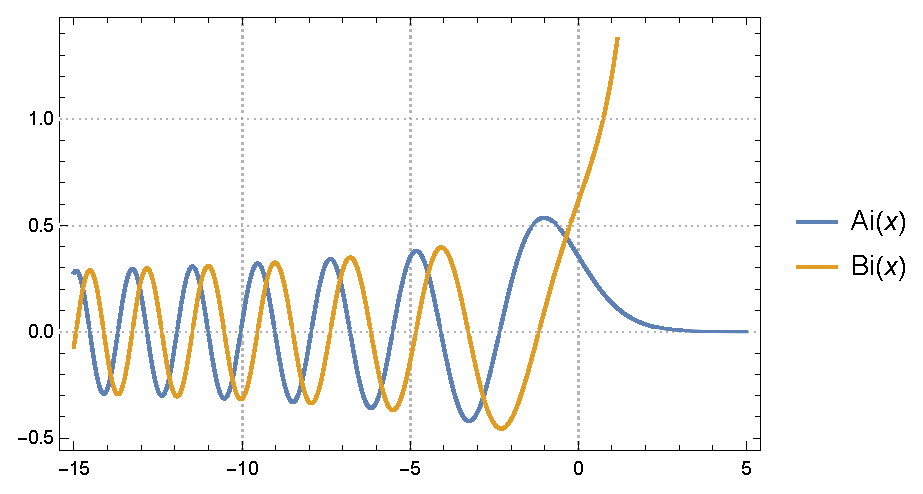
\includegraphics[scale=0.85]{fig/2-7-1.eps}
        \caption{Airy function}
    \end{figure}
    注意到$\lim\limits_{x\to +\infty}\mathrm{Bi}(x)=+\infty$, 无法归一化, 所以量子力学中我们会舍去$\mathrm{Bi}(x)$。

    还可以利用反常积分直接定义艾里函数:
    \begin{equation*}
        \mathrm{Ai}(x)=\frac{1}{\pi}\int_{0}^{+\infty}\cos\left(\frac{t^3}{3}+xt\right)dt
    \end{equation*}
    \begin{equation*}
        \mathrm{Bi}(x)=\frac{1}{\pi}\int_{0}^{+\infty}\left[\exp\left(-\frac{t^3}{3}+xt\right)+\sin\left(\frac{t^3}{3}+xt\right)\right]dt
    \end{equation*}
    
    而且$\mathrm{Ai}(x)$是正交归一的, 这也印证了量子力学本征态之间的正交归一关系:
    \begin{equation*}
        \int_{-\infty}^{+\infty}\mathrm{Ai}(t+x)\mathrm{Ai}(t+x)\mathrm{d}t=\delta(x-y)
    \end{equation*}